
For now what follows only deals with viscous behavior. The reader is referred to Barnes \cite{barn99}
for a discussion and review of non-linear viscous rheologies. 


\subsubsection{Linear viscous aka Newtonian} \index{Newtonian fluid}

Simply put, a Newtonian fluid is a fluid in which the viscous stresses at every point are linearly proportional 
to the local strain rate.
Mathematically speaking, this means that the fourth-order tensor ${\bm C}$ relating the viscous stress 
tensor to the strain rate tensor does not depend on the stress state and velocity of the flow.
\[
{\bm \tau}={\bm C} : \dot{\bm \varepsilon}
\]

One very often make sthe assumption that the fluid is isotropic, i.e. its mechanical properties are the 
same along any direction. As a consequence the fourth order viscosity tensor 
${\bm C}$ is symmetric and will have only two independent real parameters: 
a bulk viscosity coefficient, that defines the resistance of the medium to gradual uniform compression; 
and a dynamic viscosity coefficient $\eta$ that expresses its resistance to gradual shearing, 
(we here neglect the so-called rotational viscosity coefficient which results from a coupling between the fluid flow and the rotation of the individual particles). %wiki

Rather logically we denote by non-Newtonian fluids with are not Newtonian, i.e. their viscosity (tensor)
depends on stress. Such fluids are part of our daily life, e.g. honey, toothpaste, paint, blood, and shampoo.
They are also sometimes denoted as Generalized Newtonian Fluid \index{Generalized Newtonian Fluid}. 
 


%------------------------------
\subsubsection{Power-law model}
\index{Power-law model}

One of the simplest non-Newtonian viscosity model is the power-law model:
\begin{equation}
\eta = K \dot{\varepsilon}_{II}^{(n-1)/2}
\end{equation}
where $\dot{\varepsilon}_{II}$ is the second invariant of the strain rate tensor as defined in 
Section~\ref{sec:invariants}, and $n$ and $K$ are parameters. $n$ is called the power-law index.

Note that a Newtonian viscosity is recovered when $n=1$. Also $n$ and $K$ may depend on temperature
\cite[p339]{reddybook2}.

\Literature \cite{enmo97}

%------------------------------
\subsubsection{Carreau model}
\index{Carreau model} 

Note that this model is sometimes called Bird-Carreau in the literature. \index{Bird-Carreau model}
As explained in \cite{reddybook2}, the power-law model poses no restriction on 
how small or large the viscosity may become, which may prove problematic once 
implemented as it can lead to runaway effects (strain rate becomes large $\rightarrow$
viscosity becomes smaller $\rightarrow$ strain rate becomes larger, etc ...).
This problem is alleviated in the so-called Carreau
\footnote{\url{https://en.wikipedia.org/wiki/Carreau_fluid}} model \cite{zifr07}. 
The viscosity is then given by
\begin{equation}
\eta = \eta_\infty + (\eta_0-\eta_\infty) \left(1 + (\lambda \dot{\varepsilon}_{e})^2 \right)^{(n-1)/2}
\end{equation}
where $\eta_0$, $\eta_\infty$, $\lambda$ and $n\in[0,1]$ are material parameters. 
$\lambda$ is called the relaxation time: it is the inverse of the shear rate at which 
the fluid changes from Newtonian to power-law behavior.

At low strain rate a Carreau fluid behaves as a Newtonian fluid with viscosity $\eta_0$.
At intermediate strain rates $\dot{\varepsilon}_{e} \lambda \sim 1$ a Carreau fluid behaves 
as a Power-law fluid. At high strain rate, a Carreau fluid behaves as a Newtonian fluid 
again with viscosity $\eta_\infty$.
 
\begin{center}
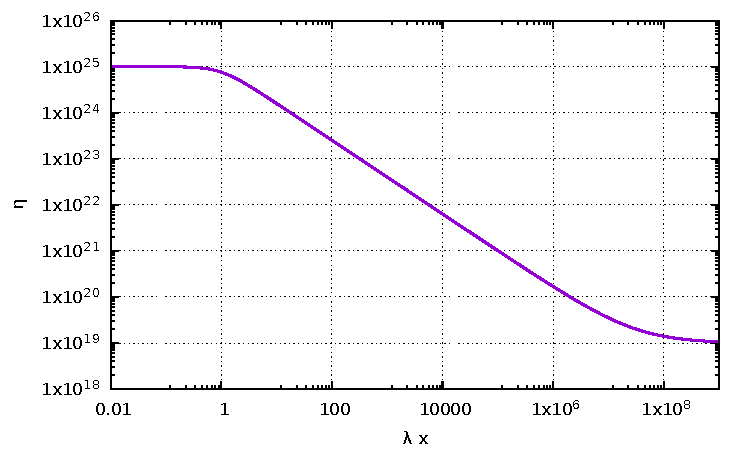
\includegraphics[width=8cm]{images/rheology/carreau/carreau.pdf}\\
{\small Carreau model effective viscosity as a function of the product $\lambda \dot{\varepsilon}_{e}$}
\end{center}

\begin{center}
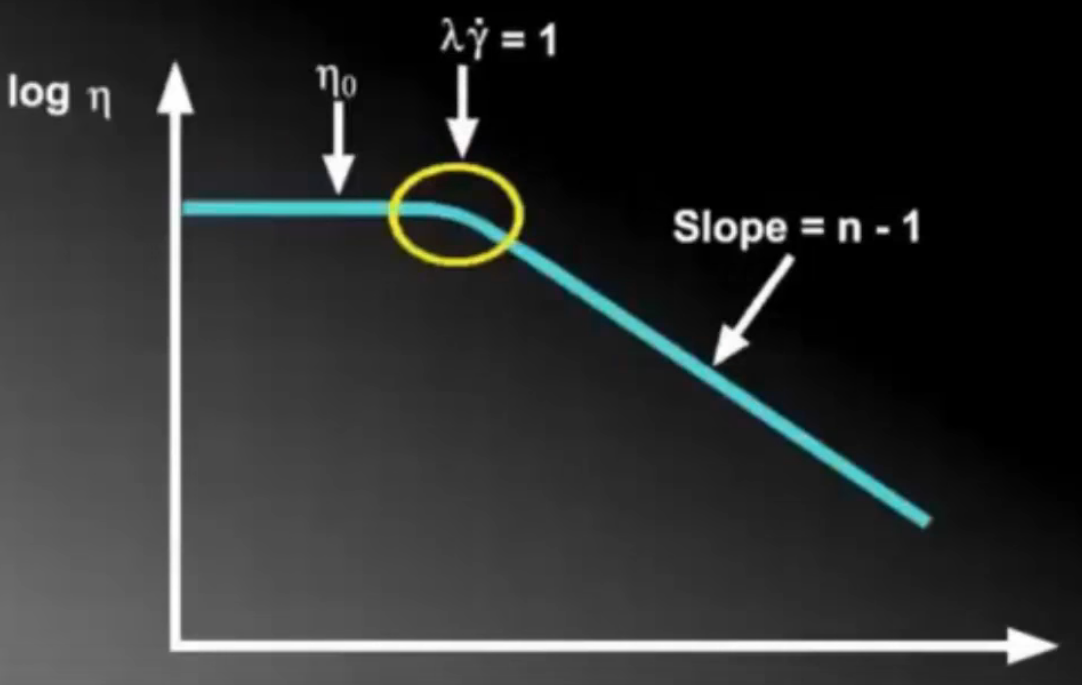
\includegraphics[width=6cm]{images/rheology/carreau/carreau1.png}\\
\url{https://youtu.be/qErs5zZV4BQ}
\end{center}

Note that the (Bird)-Carreau-Yasuda model \cite{osru14} is very similar to the standard (Bird)-Carreau:
\begin{equation}
\eta = \eta_\infty + (\eta_0-\eta_\infty) \left(1 + (\lambda \dot{\varepsilon}_{e})^a \right)^{(n-1)/a}
\end{equation}
\index{Bird-Carreau-Yasuda model}



%------------------------------
\subsubsection{Bingham model}
\index{Bingham model}

Bingham fluids can sustain an applied stress without any motion occuring. Only when the applied stress exceeds
a yield stress $\tau_0$ then the fluid flows. This translates as follows \cite{reddybook2}:

\begin{eqnarray}
{\bm s} &=& \left(  \frac{\tau_0}{\dot{\varepsilon}} + 2 \eta_0  \right)\dot{\bm \varepsilon} \qquad \text{ if } {s}_{II}>\tau_0 \\
{\bm s} &=& {\bm 0} \qquad\qquad\qquad\qquad  \text{if } {s}_{II} \leq \tau_0 
\end{eqnarray}
When flow occurs, the effective viscosity is then given by:
\[
\eta_{eff} =  \frac{\tau_0}{\dot{\varepsilon}} + 2 \eta_0 
\]
and when the strain rate is large we recover a Newtonian behaviour.
Typical Bingham fluids are mud, slurry, toothpaste.  

When using a velocity-based FEM code, the implementation of this rheological behaviour 
is complicated by the no-flow condition under a given stress. However, our codes
require a relationship between stress and strain rate in the form of an effective viscosity
which cannot be zero. 
This difficulty can be circumvented by implementing Bingham fluids as follows \cite{reddybook2}:

\begin{eqnarray}
{\bm s} &=& \left(  \frac{\tau_0(1-\eta/\eta_r)}{\dot{\varepsilon}} + 2 \eta_0  \right)\dot{\bm \varepsilon} \qquad \text{ if } {s}_{II}>\tau_0 \\
{\bm s} &=& 2 \eta_r \dot{\bm \varepsilon}  \qquad\qquad\qquad\qquad  \text{if } {s}_{II} \leq \tau_0 
\end{eqnarray}
where $\eta_r$ is a pre-yield viscosity and $\eta/eta_r<<1$ (typically 1\% or less). This is a form of 
regularisation, and we will see a similar one in the next section.

\Literature: \cite{blmi97,mizi01,maky17,syga14,bingham}

%------------------------------
\subsubsection{Herschel-Bulkley visco-plastic model}
\index{Herschel-Bulkley model}

The Herschel-Bulkley model is effectively a combination of the power-law model and 
a simple plastic model:
\begin{eqnarray}
{\bm s} &=& 2 \left(  K \dot{\varepsilon}^{n-1} + \frac{\tau_0}{\dot{\varepsilon}}\right)\dot{\bm \varepsilon} \qquad \text{ if } {s}_{II}>\tau_0 \\
\dot{\bm \varepsilon} &=& {\bm 0} \qquad\qquad \text{if }{s}_{II} \leq \tau_0 
\end{eqnarray}
in which $\dot{\varepsilon}=\sqrt{\dot{\varepsilon}_{II}}$, 
$\tau_0$ is the yield stress, $K$ the consistency, and $n$ is the flow index \cite{bemj04}.
The flow index measures the degree to which the fluid is shear-thinning ($n<1$) or shear-thickening ($n>1$).
If $n=1$ and $\tau_0=0$ the model reduces to the Newtonian model. 

The term between parenthesis above is the nonlinear effective viscosity. Concretely, the implementation goes as 
follows\footnote{\url{https://en.wikipedia.org/wiki/Herschel-Bulkley_fluid}}:
\[
\eta_{eff} = 
\left\{
\begin{array}{cc}
\eta_0 & \dot{\varepsilon}\leq \dot{\varepsilon}_0 \\ 
K \dot{\varepsilon}^{n-1} + \frac{\tau_0}{\dot{\varepsilon}} & \dot{\varepsilon} \geq \dot{\varepsilon}_0
\end{array}
\right.
\]
The limiting viscosity $\eta_0$ is chosen such that 
$\eta_0 =  K \dot{\varepsilon}_0^{n-1} + \frac{\tau_0}{\dot{\varepsilon}_0}$

A large limiting viscosity means that the fluid will only flow in response to a large applied force. 
This feature captures the Bingham-type behaviour of the fluid. 
Note that when strain rates are large, the power-law behavior dominates. 

As we have seen for Bingham fluids, the equations above are not easily amenable to implementation so that 
one usually resorts to regularisation, which is a modification of the 
equations by introducing a new material parameter which controls the exponential 
growth of stress. This way the equation is valid for both yielded and unyielded areas
\cite{blmi97,papa87,zifr07}:
\begin{equation}
\eta_{eff} = K \dot{\varepsilon}^{n-1} + \frac{\tau_0}{\dot{\varepsilon}} [1 - \exp(-m \dot{\varepsilon})] 
\end{equation}
When the strain rate becomes (very) small a Taylor expansion of the regularisation 
term yields $1- \exp(-m \dot{\varepsilon}) \sim m \dot{\varepsilon} $ so that 
$\eta_{eff} \rightarrow m \tau_0$.

\todo[inline]{Channel flow of wikipedia with analytical solution!}

\Literature: \cite{madd13}. Check dam break problem of \cite{anco09}.


\mscthesis: redo the sinking sphere in Bingham or herschel-Bulkley fluid experiment \cite{bemj04}. index{MSc Thesis}

%-------------------------------------------------
\subsubsection{The Casson model}

It is described by \cite{barn99} 
\[
\sqrt{\sigma} = \sqrt{\sigma_y} + \sqrt{\eta_p \dot{\varepsilon}_e} 
\]
or, when squaring it:
\[
\sigma = \sigma_y + \eta_p \dot{\varepsilon}_e + 2\sqrt{\sigma_p \eta_p \dot{\varepsilon}_e} 
\]
This modelled has been found to accurately describe the behaviour of synthetic based muds \cite{adlo17}. 

%-------------------------------------------------
\subsubsection{One model to rule them all?}

Let us consider the base equation
\[
\frac{\eta-\eta_\infty}{\eta_0-\eta_\infty} = 
\left[ 1+(K \dot{\varepsilon}_e)^a  \right]^{-(1-n)/a}
\]
This equation is purposefully generic and specific parameter combination choices 
allow to recover any of the above models (and more) \cite{osru14}.

%\begin{itemize}
%\item Newtonian:  $K=0$ is sufficient
%\item power-law: $\eta << \eta_0$, $\eta >> \eta_\infty$, $a=1$:
%\end{itemize}
Similar conclusions are reached in the following video:
\begin{center}
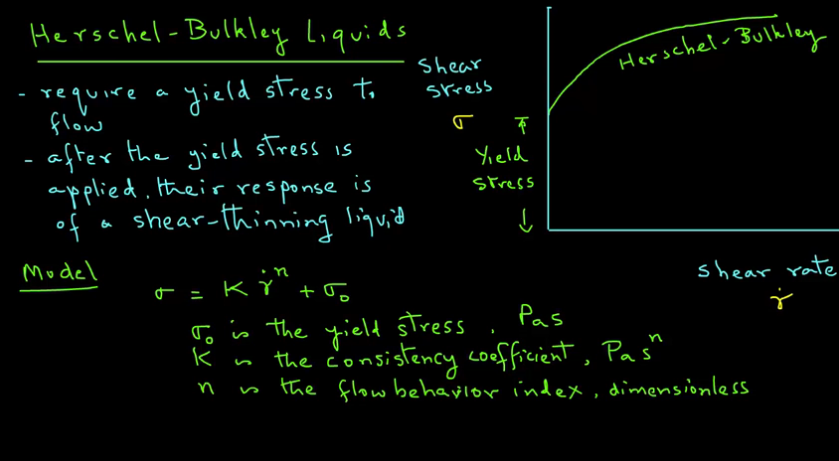
\includegraphics[width=6cm]{images/rheology/hbyoutube}\\
\url{https://youtu.be/dVCb11dZR7Y}
\end{center}



%-------------------------------------------------
\subsubsection{Dislocation and Diffusion creep}
\index{Dislocation creep}
\index{Diffusion creep}

The standard dislocation creep effective viscosity is given by:
\[
\eta_{eff}^{ds} = \frac{1}{2} f A^{-1/n} \dot{\varepsilon}_{II}^{(1-n)/2n} \exp \left( \frac{Q+pV}{nRT}  \right)
\] 
where $A$ is the pre-exponential scaling factor, $f$ is a scaling factor
representing viscous weakening or strengthening, $Q$ is the activation energy, 
$V$ is the activation volume, $T$ is the absolute temperature, $n$ is the power-law 
exponent, $R$ is the universal gas constant and $\dot{\varepsilon}_{II}$ is the 
second invariant of the strain rate tensor. Note that one will often find 
the same formula with the effective strain rate $\dot{\varepsilon}_e=\sqrt{\dot{\varepsilon}_{II}}$:
\[
\eta_{eff}^{ds} = \frac{1}{2} f A^{-1/n} \dot{\varepsilon}_{e}^{(1-n)/n} \exp \left( \frac{Q+pV}{nRT}  \right)
\] 
The coefficients $A,n,Q,V$ are material parameters and are obtained in the laboratory 
by means of high pressure/temperature experiments\cite{kawu93}. Unfortunately 
these experiments cannot be run at Earth-like strain rate values ($\sim 10^{-15}\text{s}^{-1}$)
so that extrapolations must be carried out over several orders of magnitude to 
arrive at values we can use in our numerical models. 
The 1/2 factor arises from the relationship between deviatoric stres and strain rate which 
incolves a factor 2.

The factor $f$ is in fact a tuning parameter used to explore end members (e.g. 'weak crust' 
vs 'strong crust'), see discussion in the supplementary material in \cite{hube11}. 
This approach has been extensively used by the SOPALE users community, see 
for instance \cite{wabj08,wabj08b,wabj08c,grpy12}.



Furthermore, we know that several other factors will strongly affect the rheology:
\begin{itemize}
\item water content, or as often mentioned: 'dry' vs 'wet'. Following \cite{kawu93}, 
dry means water-free and wet means water-saturated conditions.
\begin{center}
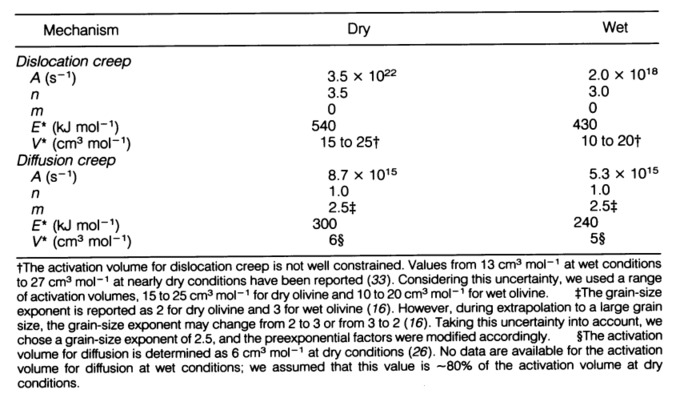
\includegraphics[width=8cm]{images/rheology/kawu93}\\
{\small Taken from Karato and Wu \cite{kawu93}.}
\end{center}
\Literature: \cite{qubu14} and refs therein for the effects of water
migration on models of subduction dynamics.

\item composition: while one typically assigns olivine properties to the mantle in models, 
the mineral olivine\footnote{\url{https://en.wikipedia.org/wiki/Olivine}} 
is actually a magnesium iron silicate with the formula (Mg$^{2+}$, Fe$^{2+}$)$_2$SiO$_4$.
and the ratio of magnesium to iron varies between the two endmembers of the solid solution series: 
forsterite (Mg-endmember: Mg$_2$SiO$_4$) and fayalite (Fe-endmember: Fe$_2$SiO$_4$).

\item grain size: this only affects diffusion creep mechanisms \cite{kawu93}. 
Grain size varies over several orders of magnitude and also evolves over time and 
its evolution is affected by the ambient deformation and the deformation history.
Dannberg et al \cite{daef17} then used a diffusion creep effective viscosity 
given by:
\[
\eta_{eff}^{df} = \frac{1}{2} A_{df}^{-1} d^m \exp \left( \frac{Q_{df}+pV_{df}}{RT}  \right)
\] 
where $d$ is the (variable) grain size and $m$ the grain size exponent. Grain growth/evolution 
is usually approximated using semi-empirical expressions \cite[section~2.2]{daef17}.
Smaller grains facilitating faster creep.

The evolution of grain size in the lower mantle is discussed in detail by Solomatov 
\cite{solo01,soet02,sore08}.



\Literature: \cite{mube18}

\item anisotropy, LPO: 

\item phase changes:

\end{itemize}

\begin{remark}
It is not uncommon to find in the literature effective viscosity formulations written as a function 
of $B$ with $B=A^{-1/n}$ \cite{wabj08,wabj08b,wabj08c}. Also, this $B$ coefficient often contains the conversion 
factor of the next remark.
\end{remark}

\begin{remark}
uniaxial stuff 
An additional coefficient is added to the effective viscosity formula(s ??) \cite{grpy12,grpy13}.
 
\[
3^{-(1+n)/2n}2^{(1-n)/n}
\] 
\cite{ranalli}
\end{remark}

\paragraph{Combining diffusion and dislocation creep} It is rather common in 
the computational geodynamics to combine both viscosities into one so-called
'effective viscous viscosity' (as opposed to the so-called 'effective plastic viscosity').
The harmonic average is then used:
\[
\eta_{eff} = \frac{\eta_{df}\eta_{ds}}{\eta_{df}+\eta_{ds}} 
=\left( \frac{1}{\eta_{df}}+\frac{1}{\eta_{df}} \right)^{-1}
\]



\Literature \cite{budr08} 


%------------------------------
\subsubsection{Peierls creep}
\index{Peierls creep}

Looking at the literature, there seems to be many formulations for the Peierls creep deformation
mechanism but it it appears that a standard formulation for the Peierls creep writes:
\[
\dot{\epsilon} = A \sigma^n \exp \left[ -\frac{Q+pV}{RT} \left(1-(\frac{\sigma}{\sigma_P})^k\right)^q  \right]
\]
and it seems common to take $k=1$, and $n=2$ \cite{gery10,kaka08}
\[
\dot{\epsilon} = A \sigma^2 \exp \left[ -\frac{Q+pV}{RT} \left(1-\frac{\sigma}{\sigma_P}\right)^q  \right]
\]

\Literature \cite{kayk99,basv06,buro11,faff11,gagd14,gery10,goev79,kaka08,kako09,kary01,mesk10,zhwa13,chsm18}

%-------------------------------------------------
\subsubsection{Arrhenius law}
\index{Arrhenius law}

A purely temperature-dependent dimensional Arrhenius law that emulates the temperature
dependence of viscosity in silicate rock is often employed for mantle rocks 
\cite{albe00,zhzm09,vata11,bogs13b,namu13,boba19,gult19}:
\begin{equation}
\eta(T)=\eta_0 \exp \left( \frac{Q}{R}(\frac{1}{T}-\frac{1}{T_0}) \right)
\end{equation}
where $\eta_0$ is a reference viscosity and $T_0$ its corresponding reference 
temperature.

It can also account for pressure effects as in \cite{lorg18} where the
diffusion creep viscosity (under the assumption of homogeneous grain size)
is temperature- and pressure-dependent:
\[
\eta(T)=\eta_0 \exp \left( \frac{1}{R}(\frac{Q-pV}{T}-\frac{Q}{T_0}) \right)
\]
(I find the minus sign rather suspicious)

%-------------------------------------------------
\subsubsection{Simple parametrisation of the mantle}

Many CITCOMs-based publications \cite{bumb10,budt14} 
have used the following (dimensionless) viscosity for the mantle:
\[
\eta(T,z) = \eta_r(r) \exp(A(0.5-T))
\]
where $\eta_r$ is a depth dependent viscosity profile (usually defined as 
discontinuous linear profiles for various shells)

The non-dimensional activation coefficient is chosen to be $A=9.2103$ in 
\cite{budt14} which leads to a temperature-induced viscosity contrast of $10^4$.

This is also called the Frank–Kamenetskii flow rule, as used in \cite{lemh17}:
\[
\eta' = \eta_0 \exp(-\theta T)
\]
where the the parameters $\eta_0$, $\theta$ account for the local chemical composition of the rock.

\index{Frank-Kamenetskii}

%-------------------------------------------------
\subsubsection{Glen's law for ice}

As it turns out, ice and rocks share similarities in terms of rheology.
Glen’s law is the most commonly used flow law for ice in glaciers and ice sheets \cite{glen55}
and it is actually a power-law type rheology:
\[
\dot{\bm \varepsilon} = A {\bm \tau}^n 
\]
with $n\sim 3$ and $A\sim 2.4\cdot 10^{-24} \text{Pa}^{-3}\cdot \text{s}^{-1}$ at $0\degree$C.
The effective viscosity is then given by
\[
\eta = \frac{1}{2 A \tau_e^{n-1}} 
\]
\begin{center}
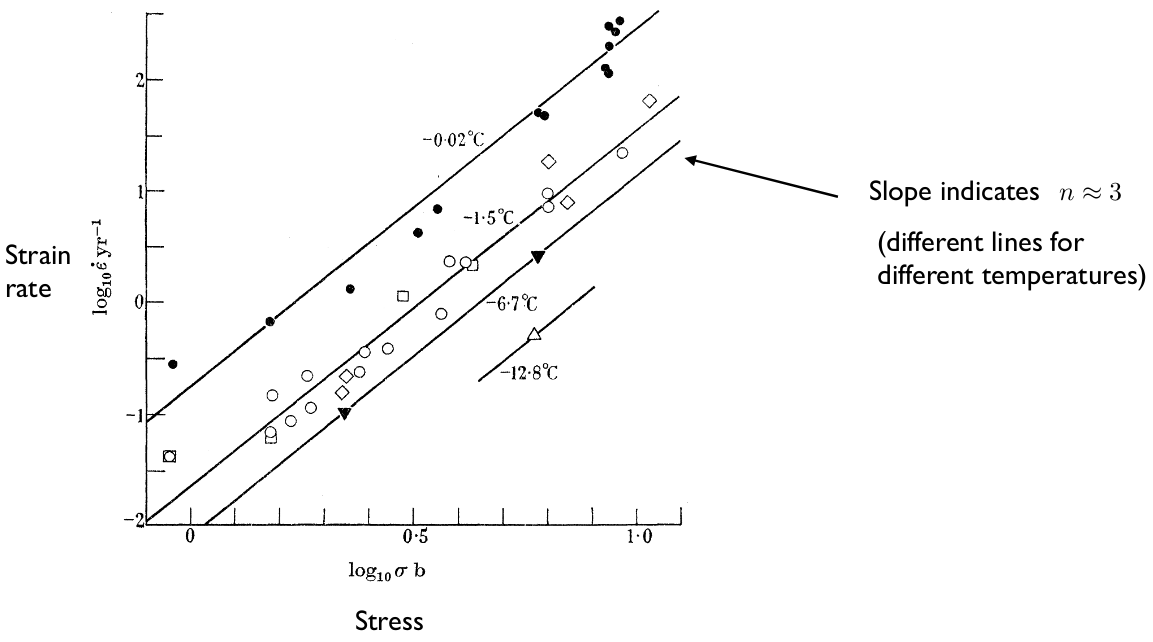
\includegraphics[height=5cm]{images/rheology/glen}
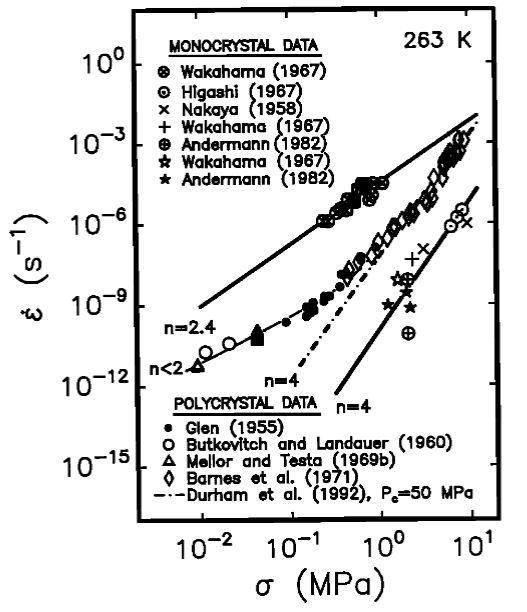
\includegraphics[height=5cm]{images/rheology/goko01}\\
{\small Left: Taken from Glen \cite{glen55}; Right: taken from \cite{goko01}.}
\end{center}
Most of these studies suggest values of the power-law exponent $n\sim 2-4$, and there seems to be 
a general indication that the exponent is lower at lower stresses.

The $A$ coefficient above has been found to depend on temperature and is reasonably described 
with an Arrhenius law:
\[
A(T)=A_0 \exp\left( -\frac{Q}{RT} \right)
\]
A standard formulation is the Paterson-Budd law with a fixed Glen exponent $n=3$ and 
a split Arrhenius term \cite{pabu82}:
\[
A=3.615 \cdot 10^{-13} \text{Pa}^{-3}\cdot \text{s}^{-1}, \qquad Q=60 \; \text{kJ}/\text{mol}, \qquad if\quad T<263\text{K} 
\]
\[
A=1.733\cdot 10^{3} \text{Pa}^{-3}\cdot \text{s}^{-1}, \qquad  Q=139 \; \text{kJ}/\text{mol}, \qquad if\quad T>263\text{K}
\]
Be careful that in these two equations the temperature T is the pressure-adjusted temperature \cite{pabu82}.


Note that $A$ is also affected by the water content and the presence of impurities. 

Finally, Glen's law is the standard rheology used for ice-sheet modelling 
but it does not account for the complex evolution of fabric and resulting anisotropy.


%...........................................
\subsubsection{Elasto-Visco-Plasticity}

\cite{anpa19} \cite{egat10}


%...........................................
\subsubsection{Anisotropic viscosity}

Following the paper by Lev and Hager (2008) \cite{leha08}, 
the anisotropic viscosity enters the equation of momentum through a 'correction'
term added to the isotropic part of the constitutive equation relating
stress and strain rate \cite{mumh02}:
\[
\sigma_{ij} = -p \delta_{ij} + 2 \eta_N \dot{\varepsilon}_{ij}  - 2(\eta_N-\eta_S)\Lambda_{ijkl}\dot{\varepsilon}_{kl} 
\]
where $\eta_N$ is the normal viscosity and $\eta_S$ is the shear viscosity. 
The fourth order tensor $\Lambda$ reflects the orientation of the directors in space, denotes by $\vec{n}$:
\[
\Lambda_{ijkl}=\frac{1}{2} (n_i n_k \delta_{lj} + n_j n_k \delta_{il} + n_i n_l \delta{kj} n_j n_l \delta_{ik} )
- 2 n_i n_j n_k n_l 
\]
Following \cite{modm03,mumh02}, the 'directors' are advected through the model and are 
analogous to particles. The directors are
vector-particles pointing normal to the easy-glide plane or layer,
thus defining the directions associated with $\eta_N$ and $\eta_S$. 
In each time
step of the calculation, the directors are advected and rotated by the
flow, and in return determine the viscosity structure for the next time
step \cite{mumc04}.


\index{MSc thesis project}

\mscthesis: redo the Rayleigh–Taylor instabilities with anisotropic lithospheric viscosity.
experiments of Lev \& Hager (2008) \cite{leha08}.
\Literature: \cite{mumh02,vatb98,mumc04,mumh02,mima04,rida78,saab84}



